\newpage
\section{Experiment - 2: The effect on IV characteristics when varying $V_{GS}$, and the device's size}
\subsection{NMOS}
\begin{figure}[H]
	\centering
	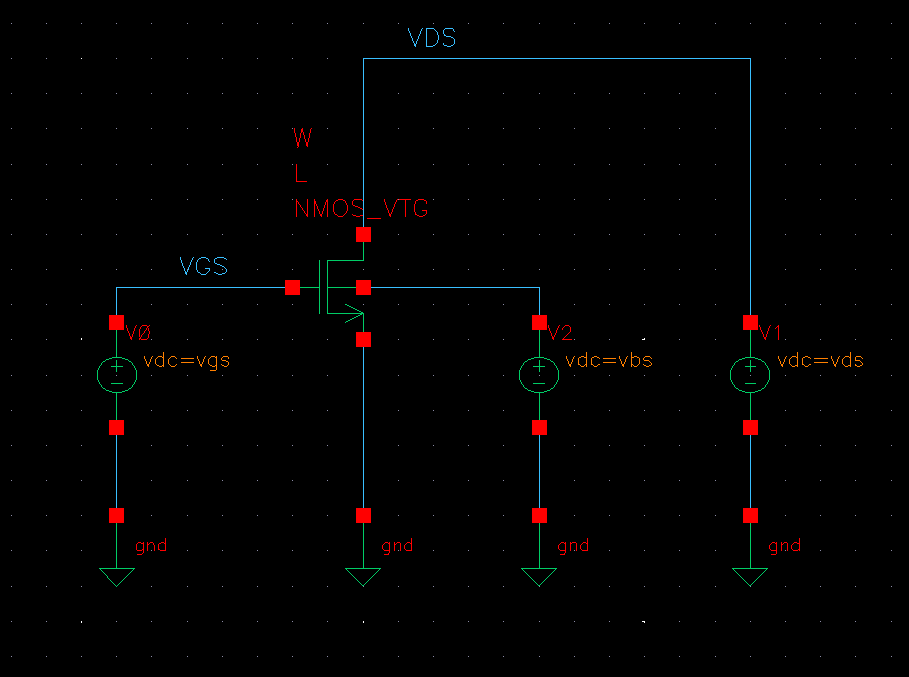
\includegraphics[width = 0.6\linewidth]{sections/pic/EX2_NMOS.png}
	\caption{Testbench NMOS\_VTG for experiment 2.}
	\label{f_ex2NMOS-schematic}
\end{figure}

\itemmini{Simulate curves $I_D$ vs $V_{GS}$ sweeping variable $V_{DS} = [0, 1](V)$ step $0.25V$.}

\begin{figure}[H]
	\centering
	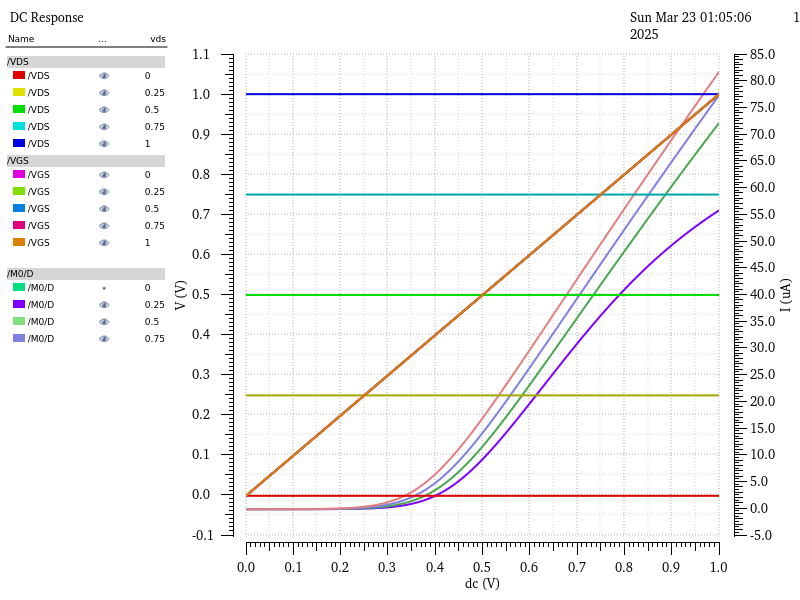
\includegraphics[width = .6\linewidth]{sections/pic/EX2_NMOS_Id&Vgs(Vds_0_1_0_25)(w)(l).png}
	\caption{$I_D$ vs $V_{GS}$ sweeping variable $V_{DS} = [0, 1](V)$ step $0.25V$.}
	\label{f_EX2_NMOS_Id&Vgs(Vds_0_1_0_25)(w)(l)}
\end{figure}

\begin{discussion}
	\item With the characteristics explained above, there is a phenomenon where as \( V_{DS} \) increases, \( V_{th} \) is observed to decrease. This is due to the phenomenon of Drain-Induced Barrier Lowering (DIBL).  
	
	\[ |V_{t} = V_{t0} - \eta V_{DS}| \]
	
	$\Rightarrow \text{The threshold voltage } V_{th} \text{ will begin to decrease as } V_{DS} \text{ increases.}$
	
\end{discussion}

\itemmini{Simulate curves $I_D$ vs $V_{DS}$ sweeping variable $V_{GS} = [0, 1](V)$ step $0.25V$.}

\begin{figure}[H]
	\centering
	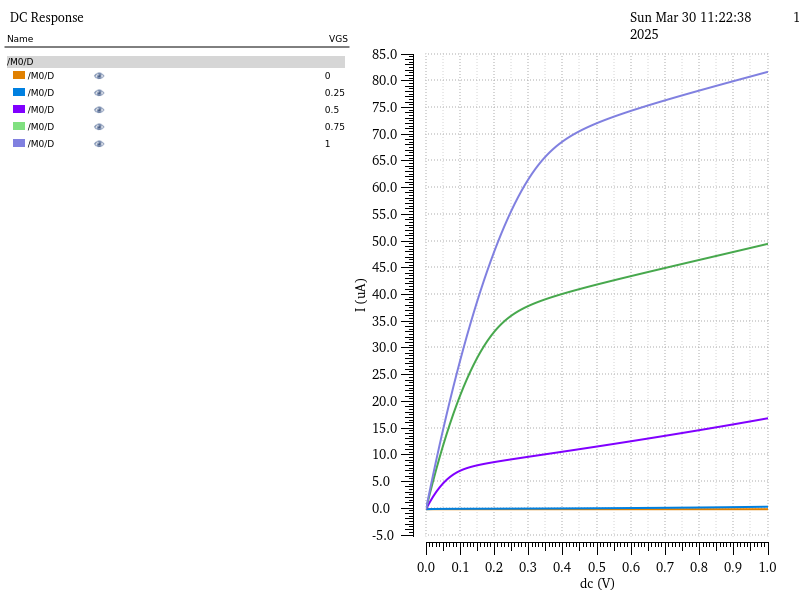
\includegraphics[width = .6\linewidth]{sections/pic/EX2_NMOS_Id&Vds(Vgs_0_1_0_25)(w)(l).png}
	\caption{$I_D$ vs $V_{DS}$ sweeping variable $V_{GS} = [0, 1](V)$ step $0.25V$.}
	\label{f_EX2_NMOS_Id&Vds(Vgs_0_1_0_25)(w)(l)}
\end{figure}

\itemmini{Simulate curves $I_D$ vs $V_{DS}$ sweeping variable $W = [30, 210](nm)$ step $30nm$.}

\begin{figure}[H]
	\centering
	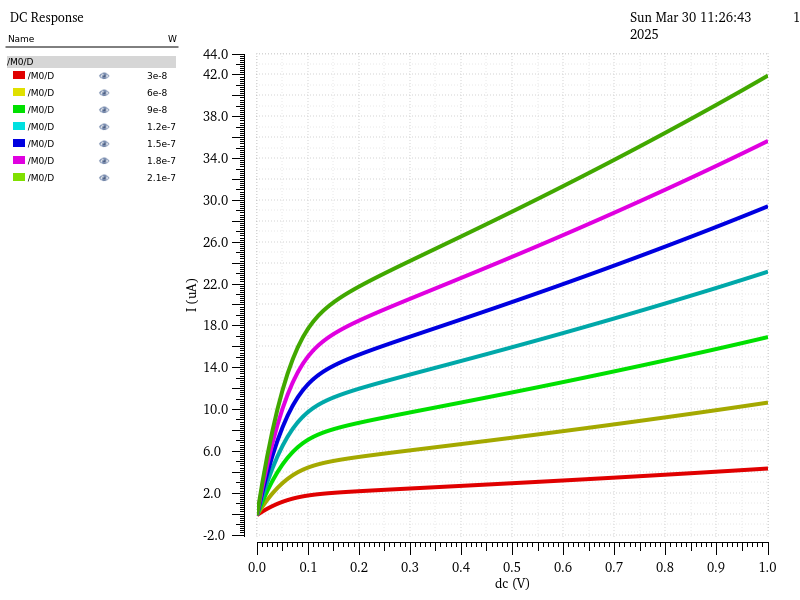
\includegraphics[width = .6\linewidth]{sections/pic/EX2_NMOS_Id&Vds(Vgs(w_30_210)(l).png}
	\caption{$I_D$ vs $V_{DS}$ sweeping variable $W = [30, 210](nm)$ step $30nm$.}
	\label{f_EX2_NMOS_Id&Vds(Vgs(w_30_210)(l)}
\end{figure}

\begin{discussion}
	\item When \( W \) increases, the slope of the \( I_{DS} \) curve in the saturation region also increases. In the figure, we can see that the curves with larger \( W \) have a steeper slope, which aligns with the theory we have learned.  
	
	\item Additionally, we can observe that as \( W \) increases, the resistance decreases, leading to a generally higher \( I_{DS} \) for the same \( V_{DS} \).
	
\end{discussion}

\itemmini{Simulate curves $I_D$ vs $V_{DS}$ sweeping variable $L = [30, 240](nm)$ step $30nm$.}

\begin{figure}[H]
	\centering
	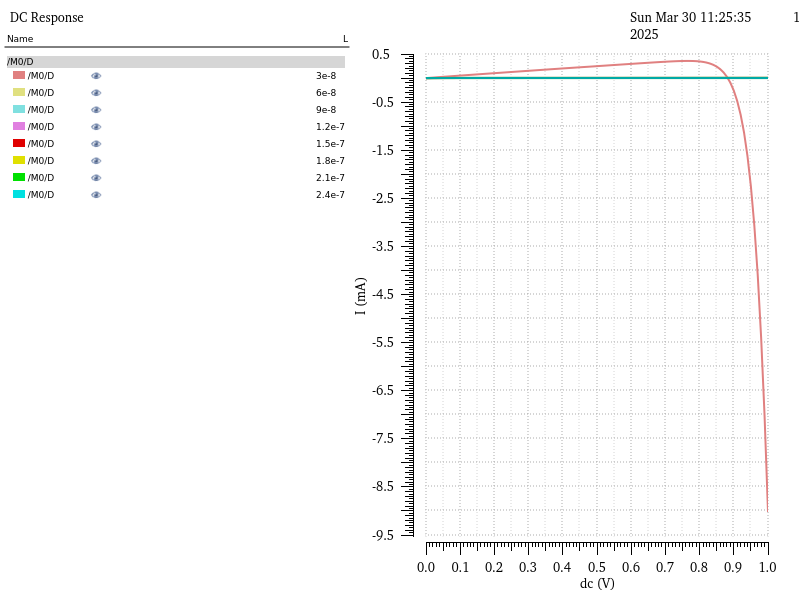
\includegraphics[width = .6\linewidth]{sections/pic/EX2_NMOS_Id&Vds(Vgs(w)(l_30_240).png}
	\caption{$I_D$ vs $V_{DS}$ sweeping variable $L = [30, 240](nm)$ step $30nm$.}
	\label{f_EX2_NMOS_Id&Vds(Vgs(w)(l_30_240)}
\end{figure}

\begin{discussion}
	\item Punch-Through Effect
	\begin{itemize}[label=+]
		\item When \( L \) is too small, the depletion regions from the drain and source can merge, preventing the MOSFET from forming a conductive channel in the usual way.
		\item The electric field from the drain can be strong enough to attract carriers back from the drain to the source, causing the drain current \( I_{D} \) to reverse (negative).
	\end{itemize}
	
	\item Strong DIBL (Drain-Induced Barrier Lowering)
	\begin{itemize}[label=+]
		\item When \( L \) is too small, the drain strongly affects the source region.
		\item The drain voltage can lower the potential barrier at the source, allowing carriers to move from the drain back to the source.
		\item If this effect is strong enough, it can lead to a reversed \( I_{D} \) current.
	\end{itemize}
\end{discussion}

\subsection{PMOS}
\begin{figure}[H]
	\centering
	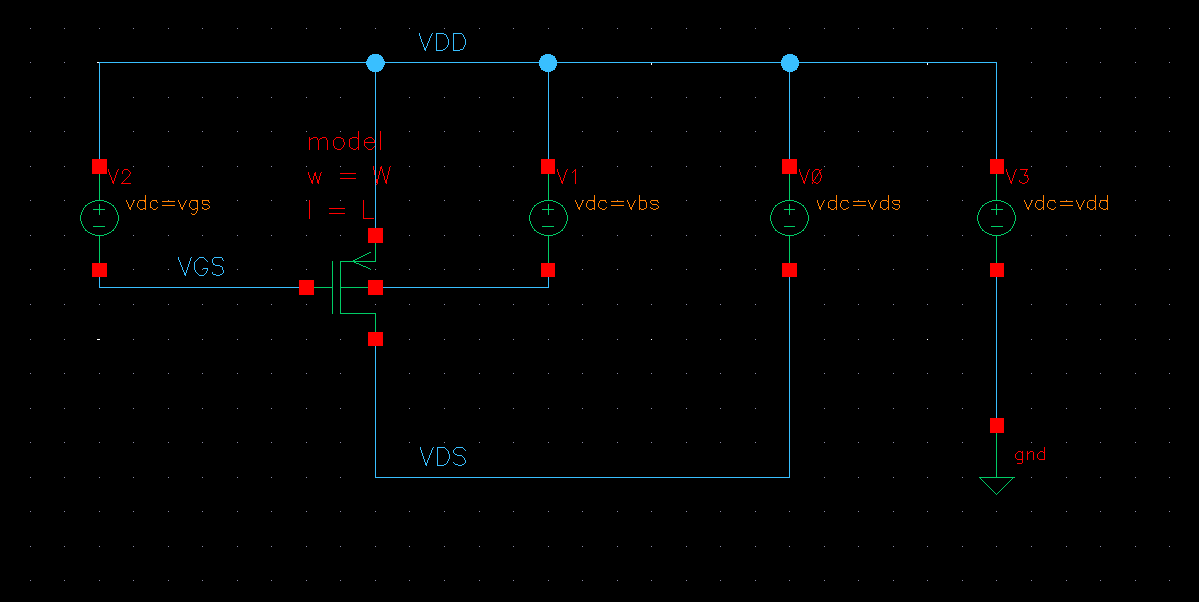
\includegraphics[width = 0.6\linewidth]{sections/pic/EX2_PMOS.png}
	\caption{Testbench PMOS\_VTG for experiment 2.}
	\label{f_ex2PMOS-schematic}
\end{figure}

\itemmini{Simulate curves $I_D$ vs $V_{GS}$ sweeping variable $V_{DS} = [0, 1](V)$ step $0.25V$.}

\begin{figure}[H]
	\centering
	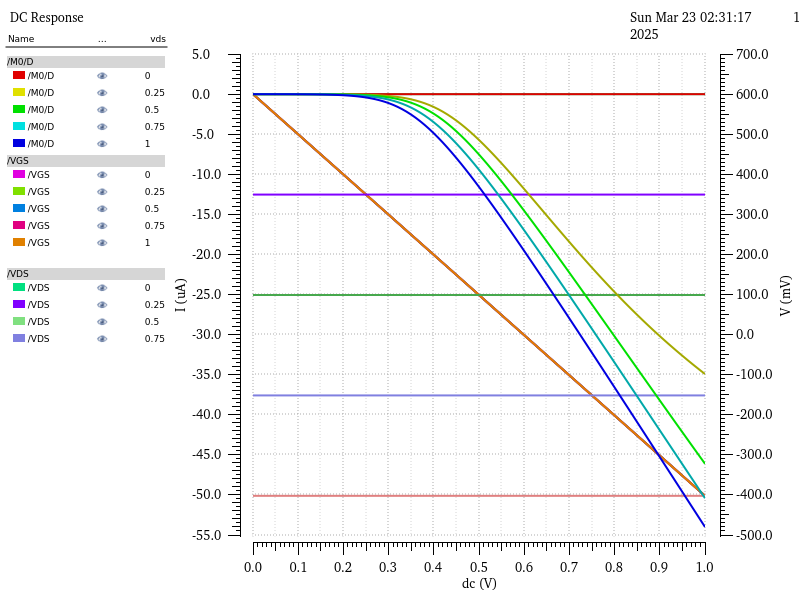
\includegraphics[width = .6\linewidth]{sections/pic/EX2_PMOS_Id&Vgs(Vds_0_1_0_25)(w)(l).png}
	\caption{$I_D$ vs $V_{GS}$ sweeping variable $V_{DS} = [0, 1](V)$ step $0.25V$.}
	\label{f_EX2_PMOS_Id&Vgs(Vds_0_1_0_25)(w)(l)}
\end{figure}

\itemmini{Simulate curves $I_D$ vs $V_{DS}$ sweeping variable $V_{GS} = [0, 1](V)$ step $0.25V$.}

\begin{figure}[H]
	\centering
	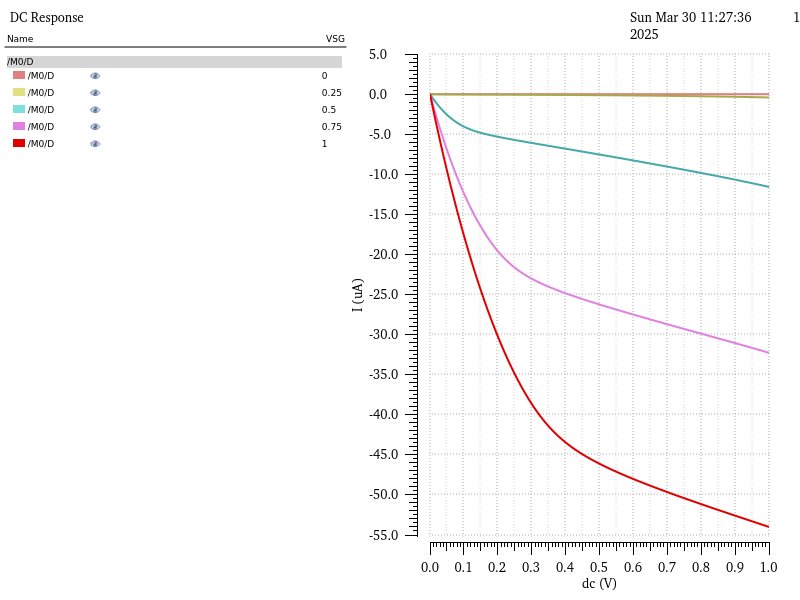
\includegraphics[width = .6\linewidth]{sections/pic/EX2_PMOS_Id&Vds(Vgs_0_1_0_25)(w)(l).png}
	\caption{$I_D$ vs $V_{DS}$ sweeping variable $V_{GS} = [0, 1](V)$ step $0.25V$.}
	\label{f_EX2_PMOS_Id&Vds(Vgs_0_1_0_25)(w)(l)}
\end{figure}

\itemmini{Simulate curves $I_D$ vs $V_{DS}$ sweeping variable $W = [30, 210](nm)$ step $30nm$.}

\begin{figure}[H]
	\centering
	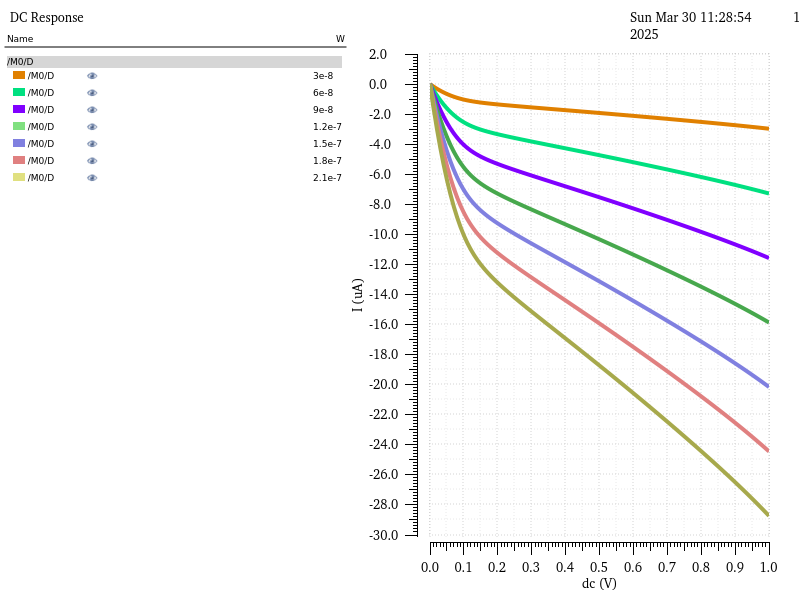
\includegraphics[width = .6\linewidth]{sections/pic/EX2_PMOS_Id&Vds(Vgs(w_30_210)(l).png}
	\caption{$I_D$ vs $V_{DS}$ sweeping variable $W = [30, 210](nm)$ step $30nm$.}
	\label{f_EX2_PMOS_Id&Vds(Vgs(w_30_210)(l)}
\end{figure}

\itemmini{Simulate curves $I_D$ vs $V_{DS}$ sweeping variable $L = [30, 240](nm)$ step $30nm$.}

\begin{figure}[H]
	\centering
	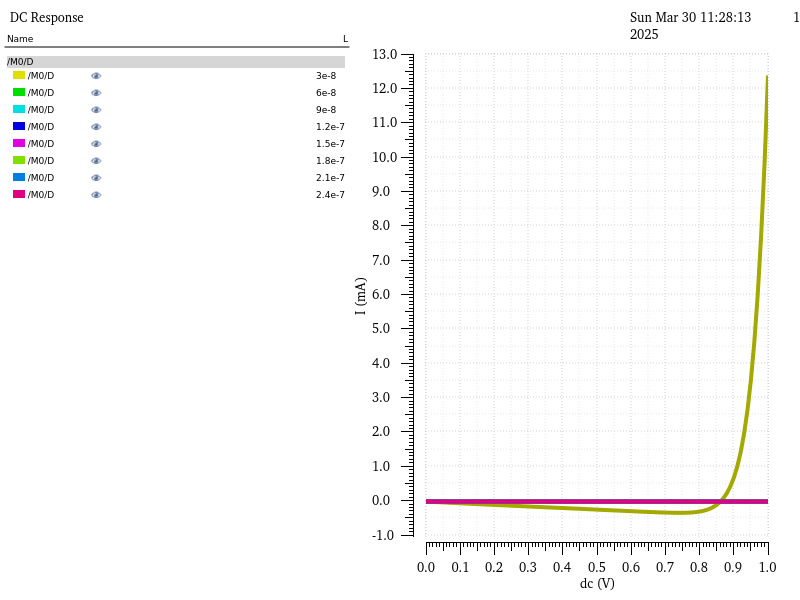
\includegraphics[width = .6\linewidth]{sections/pic/EX2_PMOS_Id&Vds(Vgs(w)(l_30_240).png}
	\caption{$I_D$ vs $V_{DS}$ sweeping variable $L = [30, 240](nm)$ step $30nm$.}
	\label{f_EX2_PMOS_Id&Vds(Vgs(w)(l_30_240)}
\end{figure}